\documentclass[border=4pt]{standalone}
\usepackage{tikz}
\usetikzlibrary{arrows,arrows.spaced}
\begin{document}
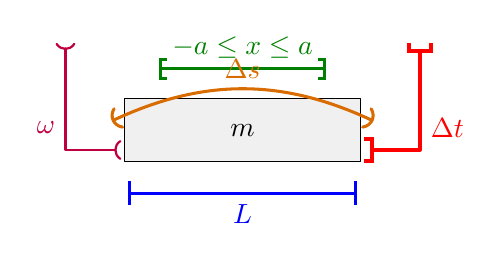
\begin{tikzpicture}[line cap=round,line join=round]
  \draw[fill=gray!12] (-1.5,-.4) rectangle (1.5,.4);
  \node at (0,0) {$m$};

  \draw[blue,line width=1.2pt,arrows={spaced |-spaced |}]
    (-1.5,-.8) -- node[below] {$L$} (1.5,-.8);
  \draw[green!50!black,line width=1pt,arrows={spaced [-spaced ]}]
    (-1.1,.78) -- node[above] {$-a\leq x\leq a$} (1.1,.78);
  \draw[orange!85!black,line width=1.1pt,arrows={spaced (-spaced )}]
    (-1.7,.1) to[bend left=25] node[above,sloped] {$\Delta s$} (1.7,.1);
  \draw[red,line width=1.35pt,arrows={spaced ]-spaced [}]
    (1.5,-.25) -| node[pos=.6,right] {$\Delta t$} (2.25,1.15);
  \draw[purple,line width=.8pt,arrows={spaced )-spaced (}]
    (-1.5,-.25) -| node[pos=.6,left] {$\omega$} (-2.25,1.15);
\end{tikzpicture}
\end{document}
